\section{General Overview of Fides}
\label{sec:general-overview-of-fides}
In this section we describe how Fides work from a high level perspective. We reference chapters and sections further into the thesis that provide more information and describe particular situations and solutions in more detail.

\begin{figure}[ht!]
    \centering
    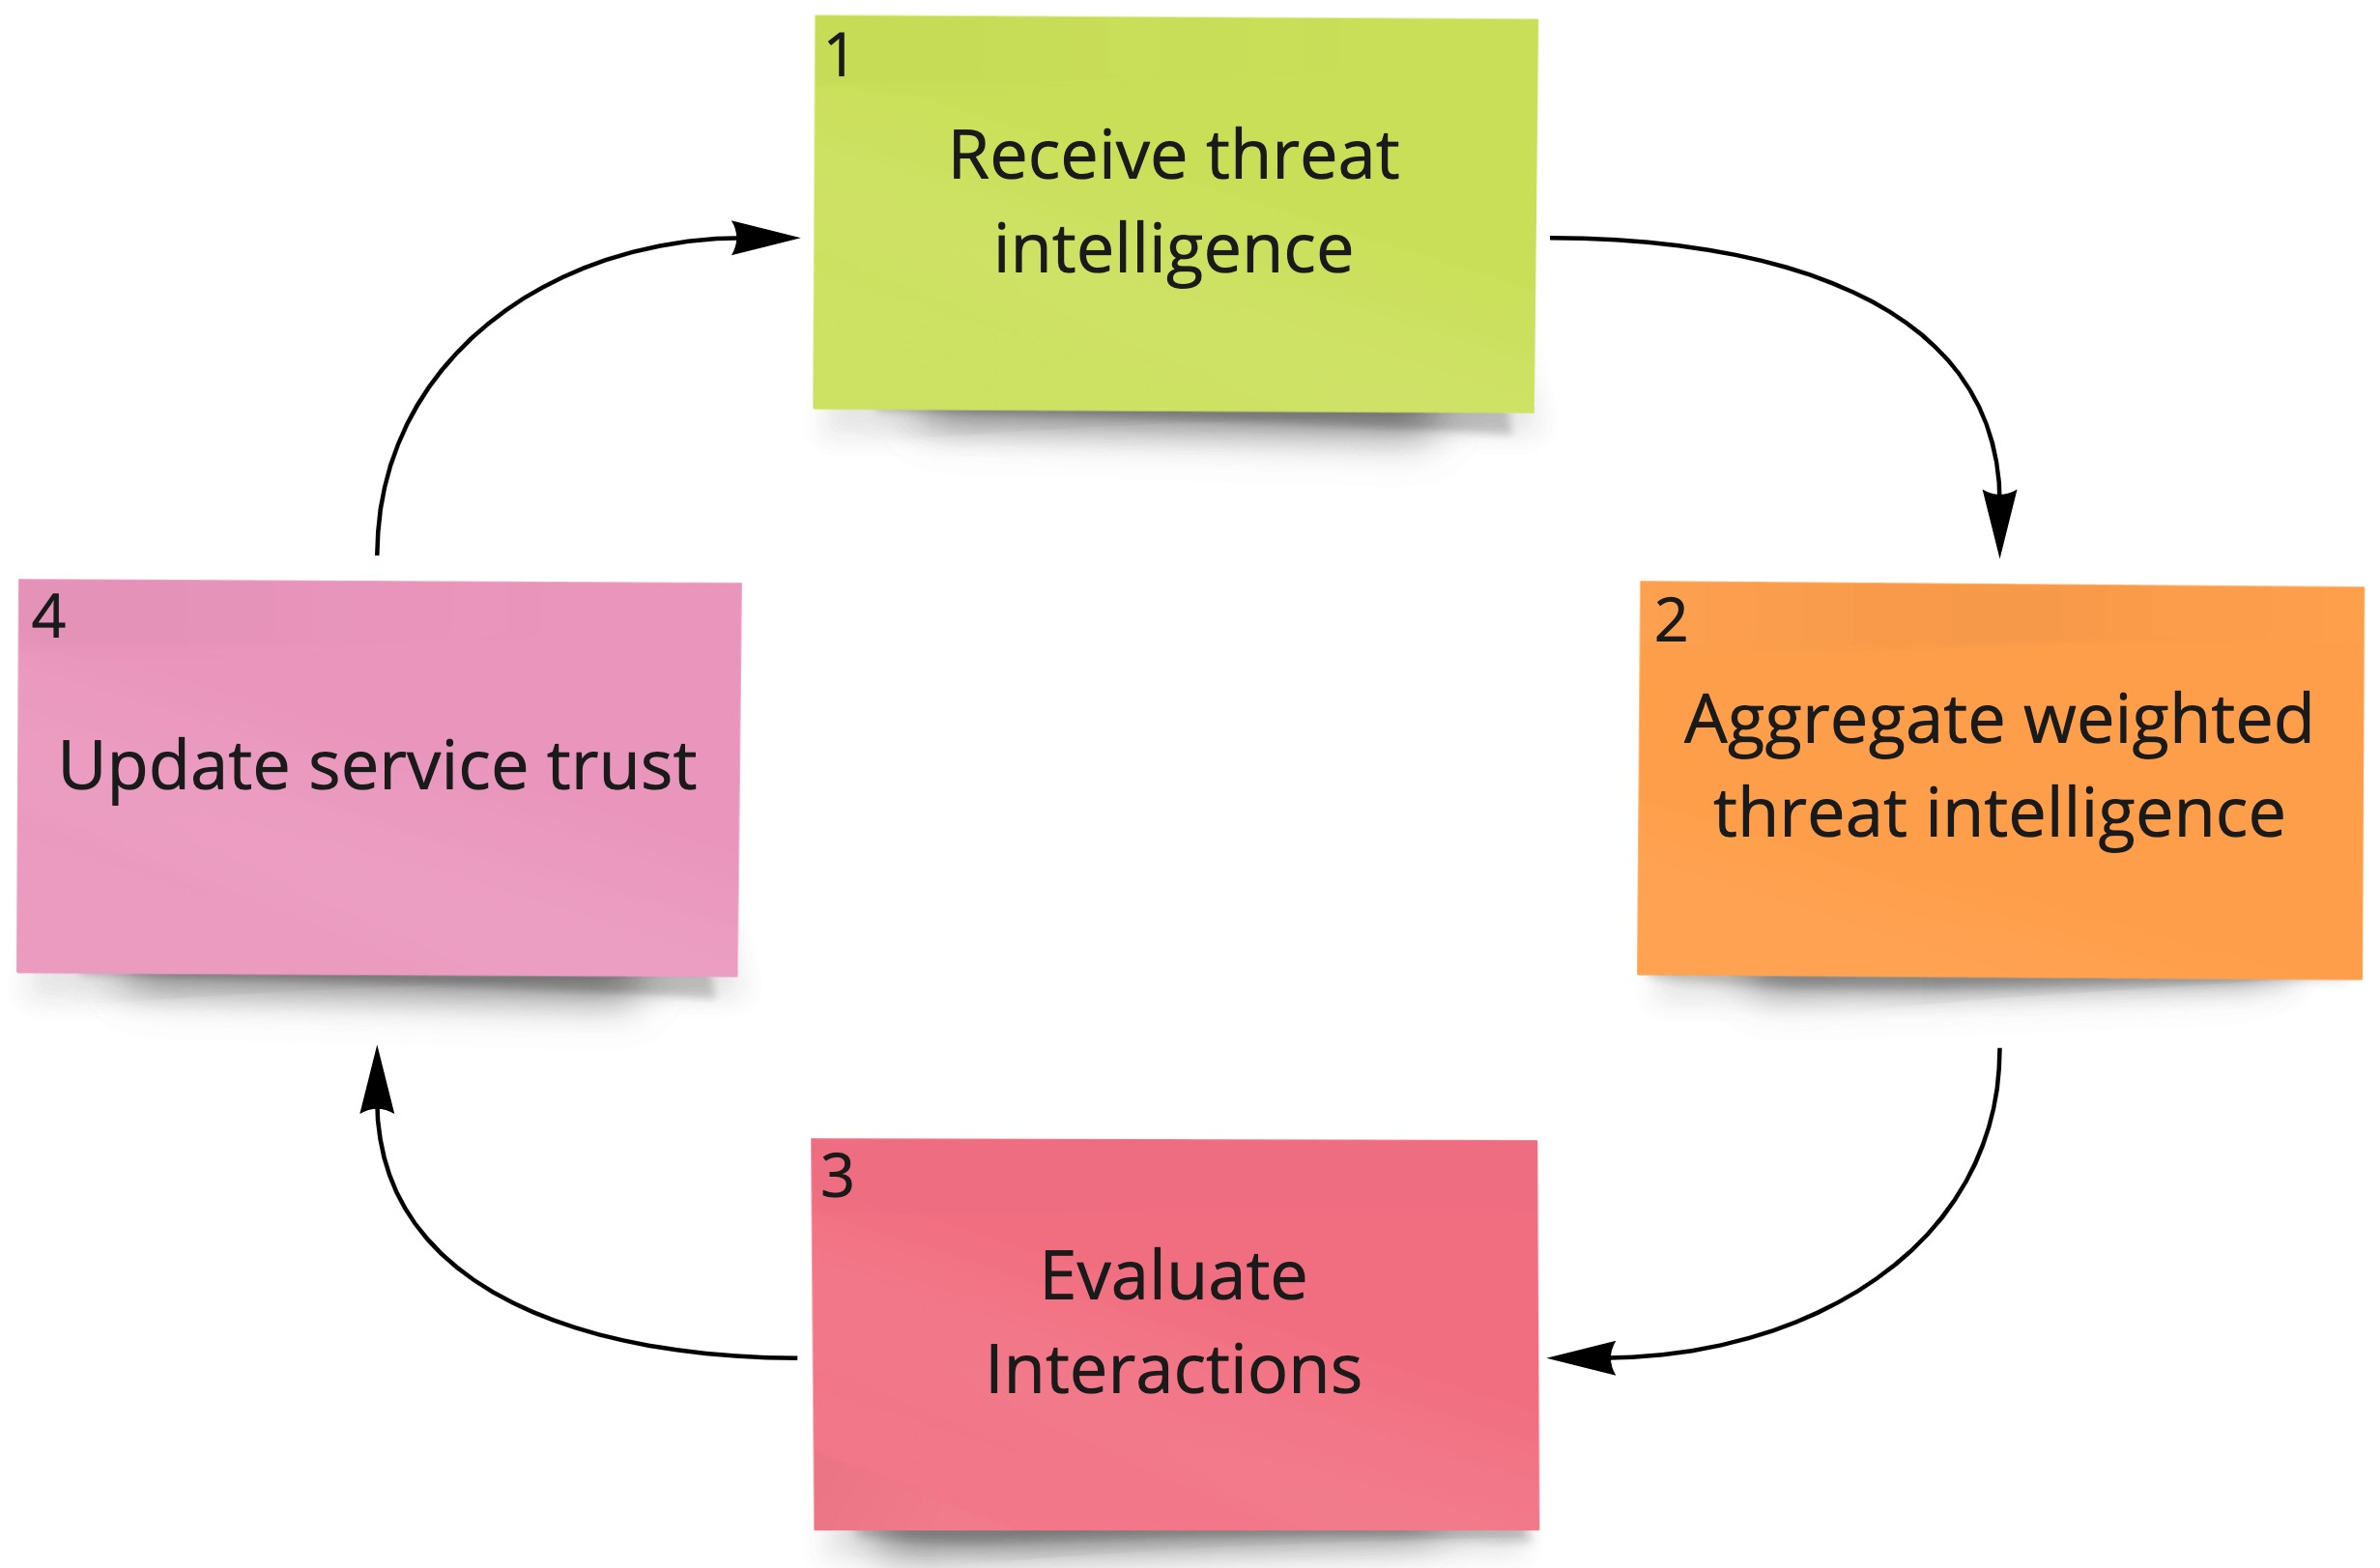
\includegraphics[width=0.75\textwidth]{assets/fides_lifecycle.jpeg}
    \caption{Generic Trust Model Life Cycle of Fides}
    \label{fig:trust-model-life-cycle}
\end{figure}

Fides operates in four general phases, which are visualized in Figure~\ref{fig:trust-model-life-cycle}.
In the first phase, a local Fides instance receives threat intelligence data from the remote peers in the network. 
How Fides receives data from the network is described in the chapter about architecture (Chapter~\ref{ch:architecture}).

In the second phase, Fides aggregates the threat intelligence data using the trust data it has for each remote peer.
In general, data from highly trusted peers have a higher impact on the final aggregated threat intelligence than the data from peers with low trust.
How does Fides do that is described in the Section~ \ref{sec:network-intelligence-aggregation}.
The aggregated threat intelligence is also sent to Slips as an output of the trust model.

In the third phase Fides evaluates the interactions with each peer.
Fides computes how much it was satisfied with threat intelligence it received from each remote peer. The evaluation does not depend on the \textit{content} of the threat intelligence and therefore is a generic method.
This satisfaction metric has then a direct influence on the trust relationship between the local and remote peers because it is used in the next step to compute trust data. 
The evaluation process and possible interaction evaluation functions are described in detail in section \ref{sec:interaction-evaluation-strategies}.

In the fourth step, Fides updates the trust data for each peer according to the satisfaction that is computed in step number three.
Computations that allow Fides to do that are described in detail in Section \ref{sec:computational-model}.

All operations including the data flow and the communication with other peers and Slips can be found on the Diagram~\ref{fig:trust-model-operational-diagram}.

\begin{figure}[h]
    \centering
    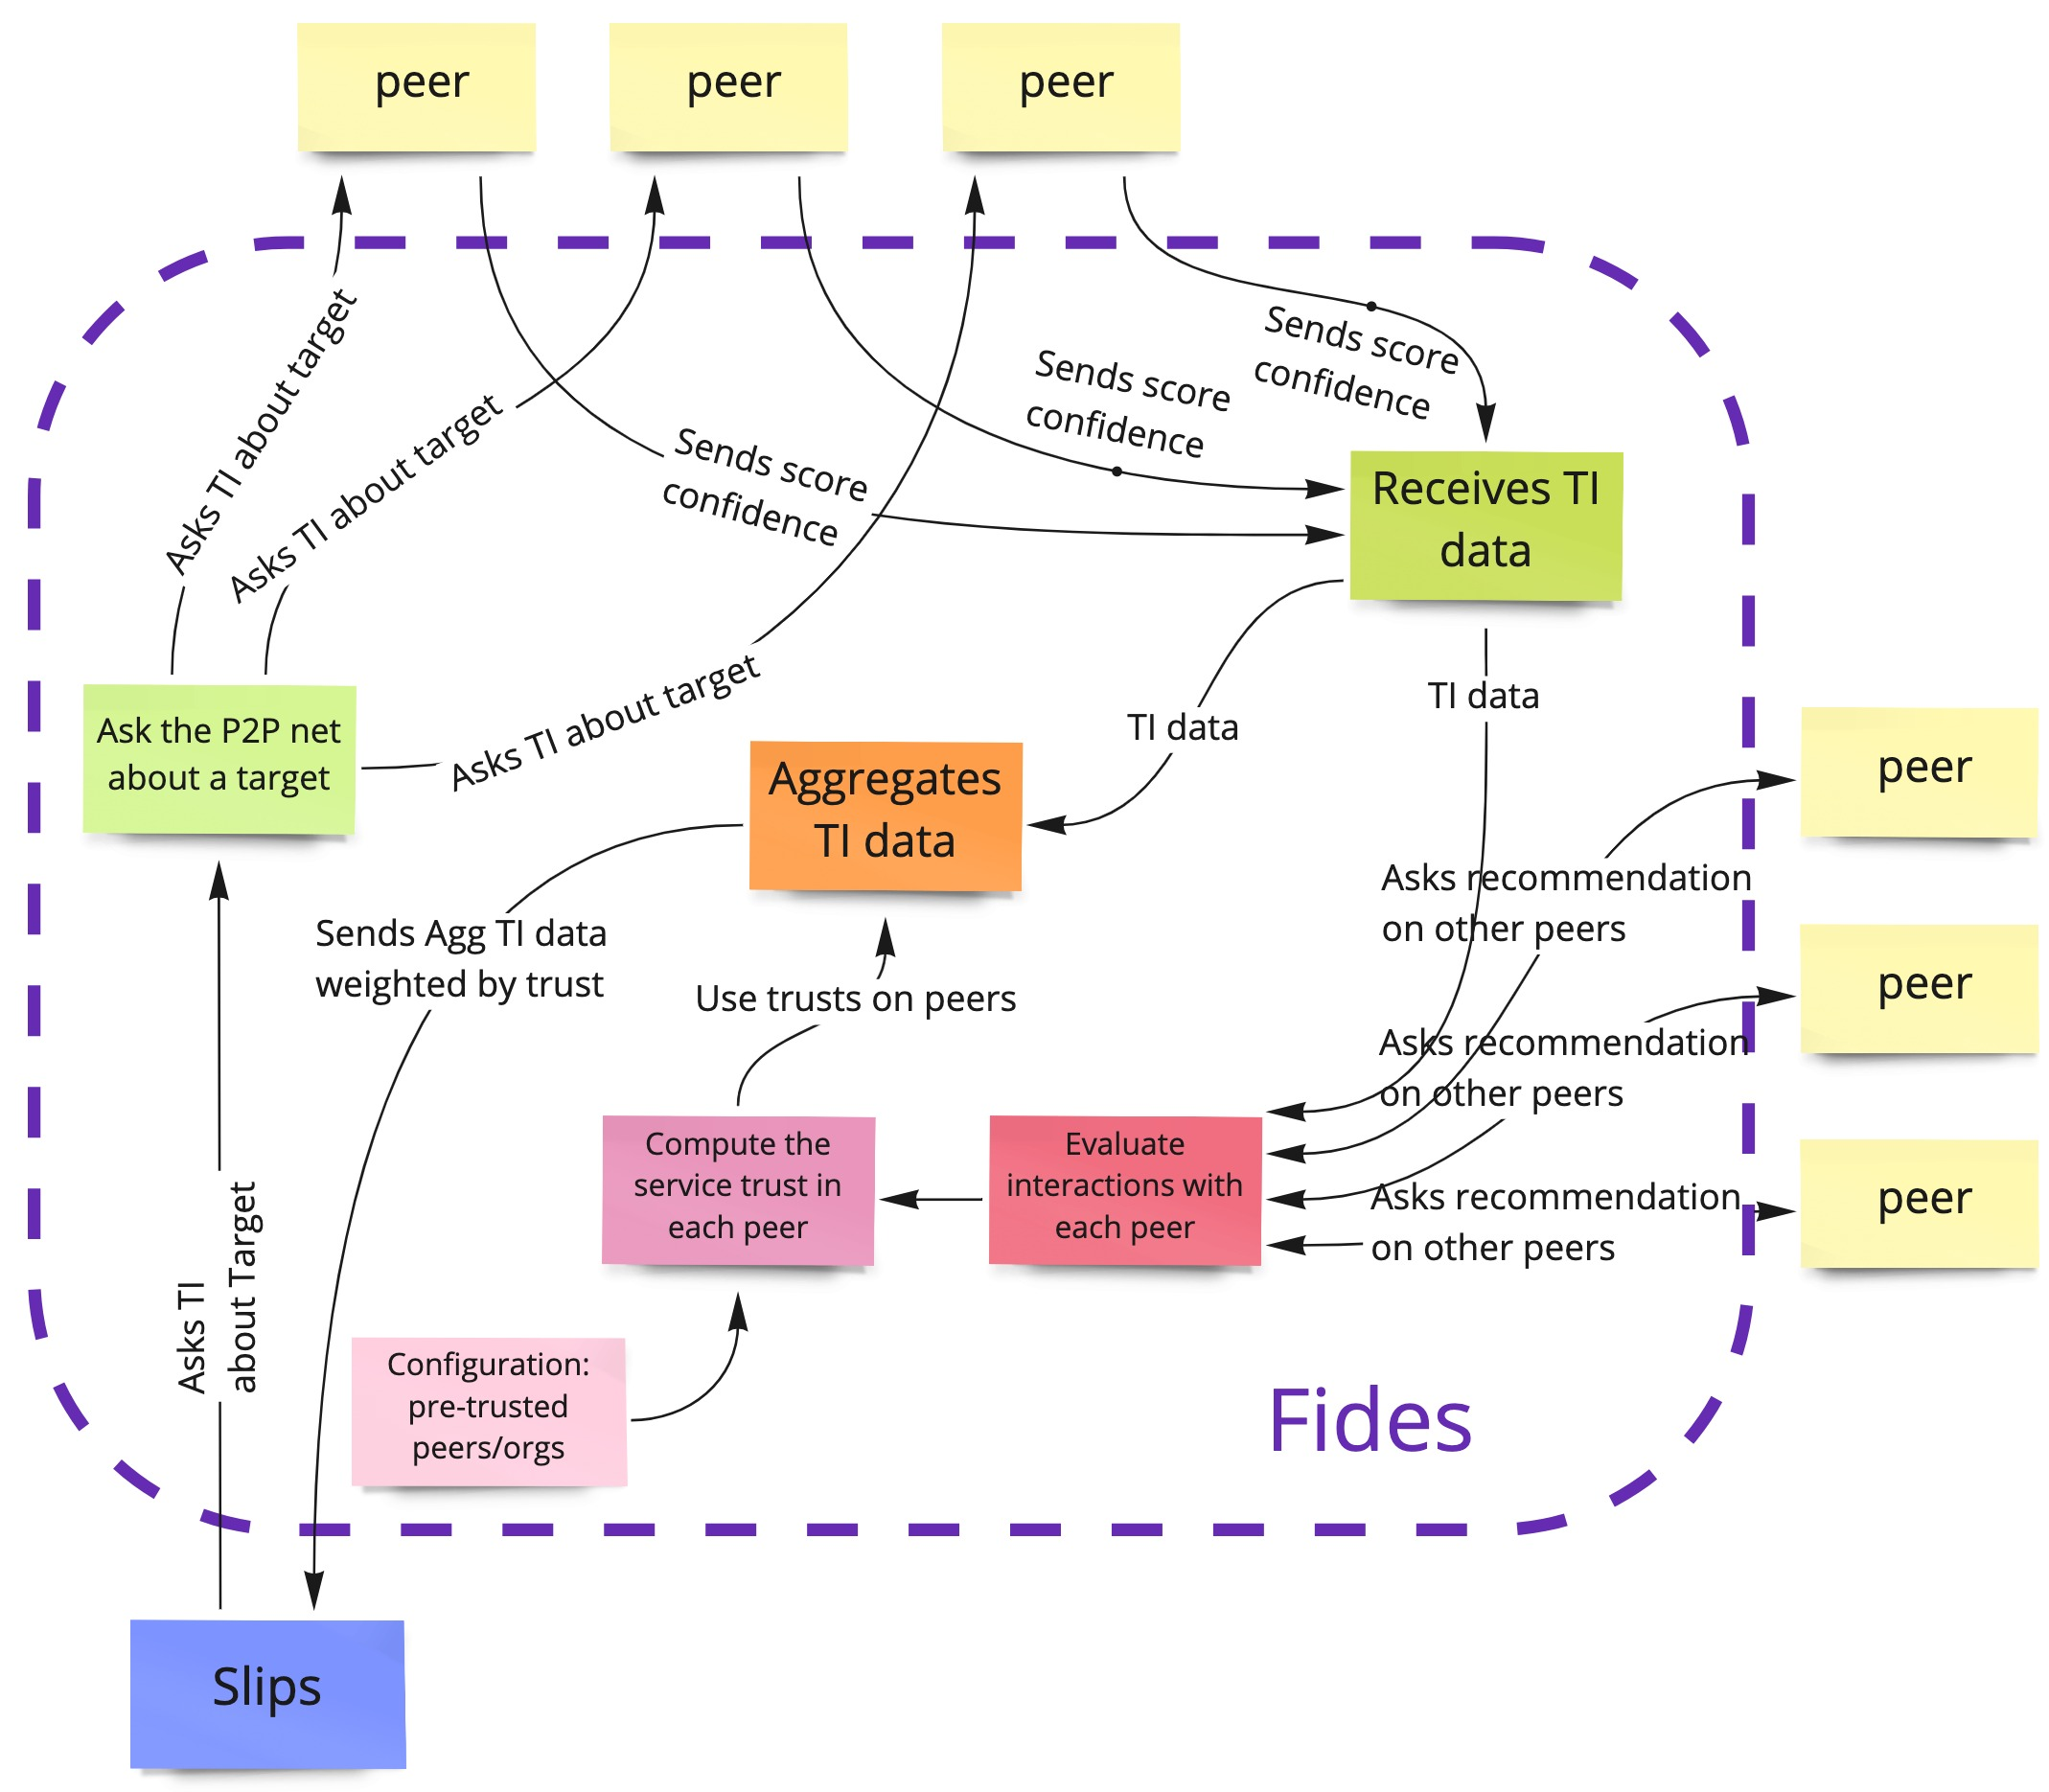
\includegraphics[width=1.0\textwidth]{assets/fides_operational_diagram.jpeg}
    \caption{Detailed Operational diagram of Fides trust model. All the inner parts of Fides are represented, together with the external parts: Slips and the P2P network.}
    \label{fig:trust-model-operational-diagram}
\end{figure}